\documentclass{math}

\usepackage{tikz}

\title{University Physics 1A}
\author{Alvin Lin}
\date{August 31st, 2017}

\begin{document}

\maketitle

\section*{Vectors}
\[ \textrm{average speed} =
  \frac{\textrm{how far}}{\textrm{how long it takes}} \]
\[ \textrm{average velocity} =
  \frac{\vec{pos_{final}}-\vec{pos_{initial}}}
  {\textrm{how long it takes}} \]
It is important to note that velocity takes the initial and final
position. One can travel some distance, but if the initial and final
position remain the same, the average velocity remains zero. This is
only the vector quantity and the displacement and speed scalars remain
the same.

\subsection*{Adding vectors in \( \R^{2} \)}
Take the following:
\begin{align*}
  \vec{v} &= \langle v_{1},v_{2}\rangle \\
  \vec{w} &= \langle w_{1},w_{2}\rangle \\
  \vec{v}+\vec{w} &= \langle v_{1}+w_{1},v_{2}+w_{2}\rangle
\end{align*}
Geometrically, this is represented as putting the tail of
\( \vec{v} \) on the head of \( \vec{w} \) and taking the vector
from the tail of \( \vec{w} \) to the head of \( \vec{v} \).
Subtraction is an analogous operation:
\begin{align*}
  \vec{v} &= \langle v_{1},v_{2}\rangle \\
  \vec{w} &= \langle w_{1},w_{2}\rangle \\
  \vec{v}-\vec{w} &= \vec{v}+(-\vec{w}) \\
  &= \langle v_{1}+(-w_{1}),v_{2}+(-w_{2})\rangle \\
  &= \langle v_{1}-w_{1},v_{2}-w_{2}\rangle
\end{align*}

\subsection*{Vector Quadrants}
\begin{center}
  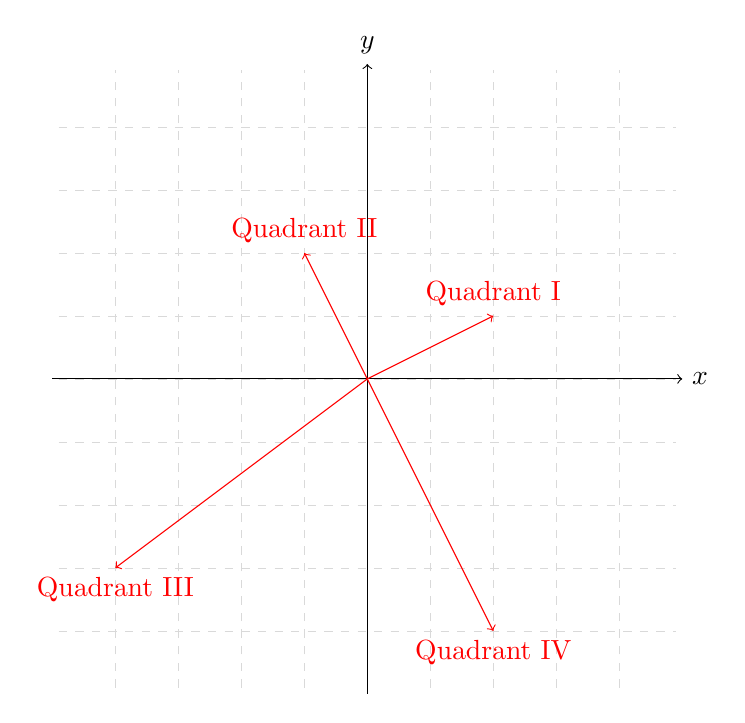
\begin{tikzpicture}[scale=0.8]
    \draw[help lines, color=gray!30, dashed] (-4.9,-4.9) grid (4.9,4.9);
    \draw[->] (-5,0)--(5,0) node[right] {\( x \)};
    \draw[->] (0,-5)--(0,5) node[above] {\( y \)};
    \draw[->,red] (0,0)--(2,1) node[above] {Quadrant I};
    \draw[->,red] (0,0)--(-1,2) node[above] {Quadrant II};
    \draw[->,red] (0,0)--(-4,-3) node[below] {Quadrant III};
    \draw[->,red] (0,0)--(2,-4) node[below] {Quadrant IV};
  \end{tikzpicture}
\end{center}

\subsection*{Polar Coordinates}
Coordinates can be represented as an angle and direction.
\begin{center}
  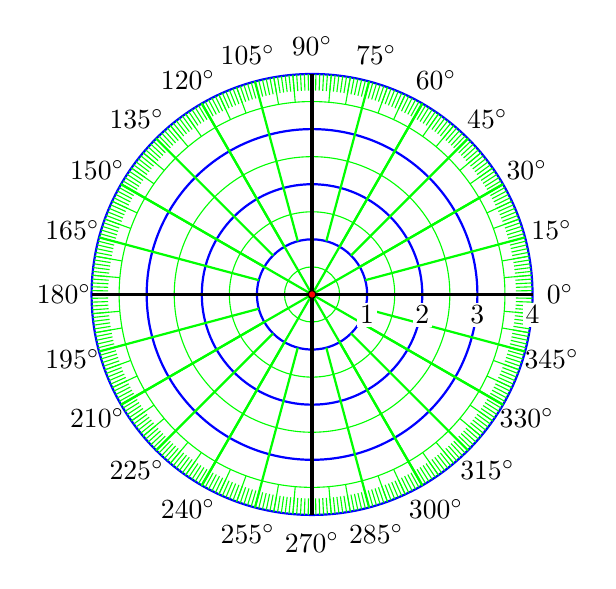
\begin{tikzpicture}[scale=0.7]
    \foreach \r in {1, 2,...,4}
      \draw[blue, thick] (0,0) circle (\r);
    \foreach \r in {0.5, 1.5,...,4}
      \draw[green, thin] (0,0) circle (\r);
    \foreach \a in {0, 1,...,359}
      \draw[green] (\a:3.7) -- (\a:4);
    \foreach \a in {0, 5,...,359}
      \draw[green] (\a:3.5) -- (\a:4);
    \foreach \a in {0, 15,...,359}
      \draw[thick,green] (\a:1) -- (\a:4);
    \foreach \a in {0, 30,...,359}
      \draw[thick,green] (0, 0) -- (\a:4);
    \foreach \r in {1, 2,...,4}
      \draw (\r,0) node[inner sep=1pt,below=3pt,rectangle,fill=white] {$\r$};
    \foreach \a in {0, 90,...,359}
      \draw[very thick] (0, 0) -- (\a:4);
    \foreach \a in {0, 15,...,359}
      \draw (\a: 4.5) node {\( \a^\circ \)};
    \draw[fill=red] (0,0) circle(0.7mm);
  \end{tikzpicture}
\end{center}
\begin{center}
  \begin{tikzpicture}[scale=0.8]
    \draw[help lines, color=gray!30, dashed] (-4.9,-4.9) grid (4.9,4.9);
    \draw[->] (-5,0)--(5,0) node[right] {\( x \)};
    \draw[->] (0,-5)--(0,5) node[above] {\( y \)};
    \draw[->,red] (0,0)--(2,2) node[above] {\( (r,\theta) \)};
    \draw[->,red] (0,0)--(-2,2) node[above]
      {\( (2\sqrt{2},135^{\circ}) \)};
  \end{tikzpicture}
\end{center}

\subsection*{Converting between polar and Cartesian coordinates}
\begin{center}
  \begin{tikzpicture}
    \draw (0,0)--(4,0) node[pos=0.5, below]{\( x \)};
    \draw (4,0)--(4,3) node[pos=0.5, right]{\( y \)};
    \draw (0,0)--(4,3) node[pos=0.5, above]{\( \vec{r} \)};
    \node[pos=1] (2,2) {\( \theta \)};
  \end{tikzpicture}
\end{center}
\begin{align*}
  x &= r\cos(\theta) \\
  y &= r\sin(\theta) \\
  r^{2} &= x^{2}+y^{2} \\
  \theta &= \arctan(\frac{y}{x})
\end{align*}
Given the unit vectors \( \vec{i} \) and \( \vec{j} \), \( \vec{r} \) can also
be represented as:
\[ \vec{r} = x\vec{i}+y\vec{j} \]

\begin{center}
  You can find all my notes at \url{http://omgimanerd.tech/notes}. If you have
  any questions, comments, or concerns, please contact me at
  alvin@omgimanerd.tech
\end{center}

\end{document}
